 
% =============================================
% ================= PREÁMBULO =================
% =============================================

\documentclass[12pt,a4paper]{article}
\usepackage[utf8]{inputenc}
\usepackage[T1]{fontenc}        % Para Tildes
\usepackage[spanish,es-tabla]{babel}
\usepackage{graphicx}
\usepackage{cite}
\usepackage{minted}



\usepackage{multicol,multirow}
\usepackage{amsmath,mathtools}
\usepackage{amsfonts}
\usepackage{amssymb}
\usepackage{adjustbox}
\usepackage[europeanresistors]{circuitikz}
\usepackage{siunitx,enumitem}
\usepackage{pdfpages}       % Para importar páginas de un pdf 
\usepackage{booktabs}
\usepackage{physics}
\usepackage[bookmarks=true,colorlinks=true,linkcolor=black,citecolor=black,menucolor=black,urlcolor=black]{hyperref} 
\usepackage[left=2cm,right=2cm,top=2cm,bottom=2cm]{geometry} 
\usepackage{float}      % Para ubicar las tablas y figuras justo después del texto
\usepackage{pdfpages}
\usepackage{svg}
\usepackage[numbered,framed]{matlab-prettifier}
\usepackage{filecontents}
\usepackage{dirtytalk}
\usepackage{cancel}
\usepackage{colortbl}
\usepackage{karnaugh-map}



\newcommand\Ccancel[2][black]{\renewcommand\CancelColor{\color{#1}}\cancel{#2}}

\usepackage{tikz}

\newcommand{\lapt}{
  \begin{tikzpicture}[baseline=-0.5ex]
    \draw (0,0) circle [radius=0.5ex];
    \draw (0.5ex,0) -- (3.5ex,0); 
    \draw[fill] (4ex,0) circle [radius=0.5ex];
  \end{tikzpicture} 
  \hspace{0.2cm}
}

\newcommand{\ilapt}{
  \begin{tikzpicture}[baseline=-0.5ex]
    \draw[fill] (0,0) circle [radius=0.5ex];
    \draw (0.5ex,0) -- (3.5ex,0);
    \draw (4ex,0) circle [radius=0.5ex];
  \end{tikzpicture}
   \hspace{0.2cm}
}



\title{Bitacora}
\date{}





% =============================================
% ================= DOCUMENTO =================
% =============================================

\begin{document} 
\maketitle


\section{8 de febrero}

\subsection{Modelo Matemático.}

Se decidió representar el modelo mátematico del tablero de la siguiente forma:


\begin{figure}[H]
\[
\begin{bmatrix}
0 & 0 & 0 & 0 &  0 &  1 \\
0 & 0 & 0 & 0 &  1 & -1 \\
0 & 0 & 0 &  1 & -1 &  1 \\
0 & 0 & 0 & -1 &  1 & -1 \\
0 & 0 & 0 &  1 & -1 &  1 \\
0 & 0 & 0 & -1 &  1 & -1
\end{bmatrix}
\quad \Longleftrightarrow \quad
\begin{bmatrix}
\phantom{\bullet} & \phantom{\bullet} & \phantom{\bullet} & \phantom{\bullet} & \phantom{\bullet} & \textcolor{blue}{\bullet} \\
\phantom{\bullet} & \phantom{\bullet} & \phantom{\bullet} & \phantom{\bullet} & \textcolor{blue}{\bullet} & \textcolor{red}{\bullet} \\
\phantom{\bullet} & \phantom{\bullet} & \phantom{\bullet} & \textcolor{blue}{\bullet} & \textcolor{red}{\bullet} & \textcolor{blue}{\bullet} \\
\phantom{\bullet} & \phantom{\bullet} & \phantom{\bullet} & \textcolor{red}{\bullet} & \textcolor{blue}{\bullet} & \textcolor{red}{\bullet} \\
\phantom{\bullet} & \phantom{\bullet} & \phantom{\bullet} & \textcolor{blue}{\bullet} & \textcolor{red}{\bullet} & \textcolor{blue}{\bullet} \\
\phantom{\bullet} & \phantom{\bullet} & \phantom{\bullet} & \textcolor{red}{\bullet} & \textcolor{blue}{\bullet} & \textcolor{red}{\bullet}
\end{bmatrix}
\]
  \caption{Equivalencia matriz tablero}
\end{figure}

La elección de este modelo, se debe a la facilidad que presenta para implementar operaciones matriciales y métodos de verificación de estado(win, lose).
Además que como se observa en el diagrama, la representación en colores que se escogió para el 1 es azul mientras que el -1, es rojo

\subsection{Herramientas de Desarrollo.}

Se planea usar como herramienta gráfica QT.
Para la implementación de la matriz de menera tentativa se planea usar alguna libreria de operaciones matriciales.

\section{10 de febrero}
\subsection{Funciones}

Para interactuar con el tablero(matriz) se definirán dos funciones
\begin{itemize}
  \item Insertar: Esta función insertará una ficha en algún elemento de la
        primera fila.

  \item Gravedad: Esta función simulará la caida de una ficha en una columna,
        siempre y cuando debajo de esta ficha exista un campo vacio.
\end{itemize}

\begin{figure}[H]
    \centering
    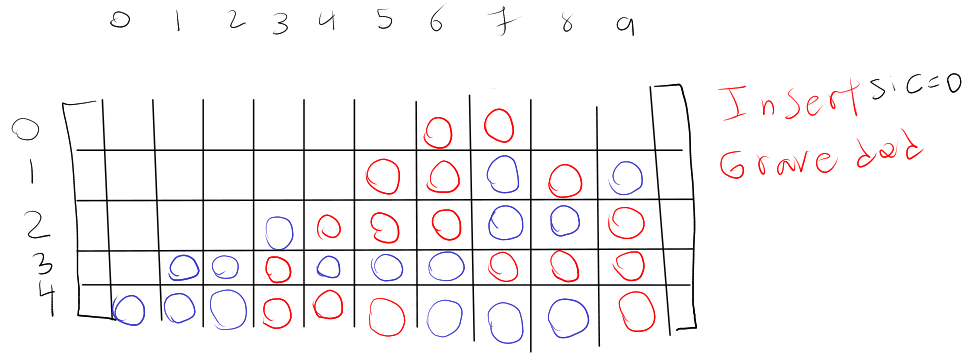
\includegraphics[width=\linewidth]{imagenes/draw.png}
    \caption{Simulación dibujada}
    \label{fig:draw_simulation}
\end{figure}


\end{document}
